\section{Introduction}
% 
\acrfull{ams} are playing a crucial role in every enterprise. They are being used/implemented for both, the physical access to company premises, online and internal resources. There are countless of different systems and providers offering such systems, ranging from simple card access systems and password log-ins to complex ones combining different types of physical and online access to resources. 

The problem of today’s access systems is that they are usually handling physical and online accesses separately, two systems have to be implemented and companies are usually specializing in providing one of those systems. Companies such as HID\footnote{\url{https://www.hidglobal.com/solutions/access-control-systems}, accessed 26 March 2019} or G4S\footnote{\url{https://www.g4s.com/en-gb/what-we-do/security-services/fire-and-security-systems/symmetry-software}, accessed 26 March 2019} are providing physical \acrshort{ams} to enterprises which allows employees to access the building, rooms, canteen or garage based on their access levels. On the other hand, there are tech companies such as Microsoft\footnote{\url{https://docs.microsoft.com/en-us/windows-server/identity/ad-ds/get-started/virtual-dc/active-directory-domain-services-overview}, accessed 26 March 2019} which offer software for managing employees’ access to online services and resources.

Therefore, there exist two mostly independent systems intended for similar use cases. These systems are either managed individually or can be interconnected, so that there is one endpoint for managing accesses. Both approaches work fine, but what if there was an \acrshort{ams} which would combine both physical and online access? What if physical access would be possible by authenticating the employee with smartcard, smartphone or authenticator key? Simply, there would be a need only for one device, with which an employee would be able to access premises as well as authenticate himself when login-in to a service. Such a system not only solves the problem of the employees’ experience and convenience of having to carry around an access card, but also a problem of security of corporate account because of passwords. The reason is that many companies has policy that requires changes of password a few times a year and therefore, employees tend to use easy to remember passwords  as well as many corporate accounts has been “hacked” by phishing attacks\cite{} Canadian Business Banking Customers Hit With Targeted Phishing, Account Takeover Attacks REF!. This can be avoided by using physical authenticators instead of passwords.

The aim of this project is to address this problem and propose a system, where physical access control and online access control is managed from the single endpoint as it can be seen in Figure~\ref{fig:IntroArchitecture}. Another very important feature introduced by this system, is the possibility of using \acrshort{fido}2 \acrshort{nfc} enabled authenticator or smartphone to access a building, rooms or printers. Both devices would work similarly to an access card which is usually given to an employee. A device needs to be swiped in front of the reader or connected to a reader wirelessly, using \acrshort{ble} in case of smartphone, which allows or deny access. It is common these days, that employees get to use many online services with their corporate account. To avoid passwords, technology called \acrshort{fido}2 aims to get rid of passwords when logging into account by using an authenticator, either a physical key device or smartphone. This allows “strong authentication” (REF! Why Strong Authentication is a Critical Requirement for Improving Critical Infrastructure Cybersecurity). The only thing the employee needs to type in when logging-in is the user ID and then he needs a \acrshort{fido}2 authenticator which authenticates him, at least in our system. Because of that, the employee has no longer to carry an access card with him, and only needs smartphone or authenticator when accessing physical premises of enterprise, as well as it empowers him to “forget” about passwords when logging-in into online services by using the same smartphone and authenticator.

Secondary aim of this system lies in the access management, which grants or denies the entry or use of a service for an employee. To facilitate this, policies and role-based access will be implemented, which allows for assigning each employee a role/s and to create policies by which the access will be granted or denied automatically.

\begin{figure}[ht]
    \centering
    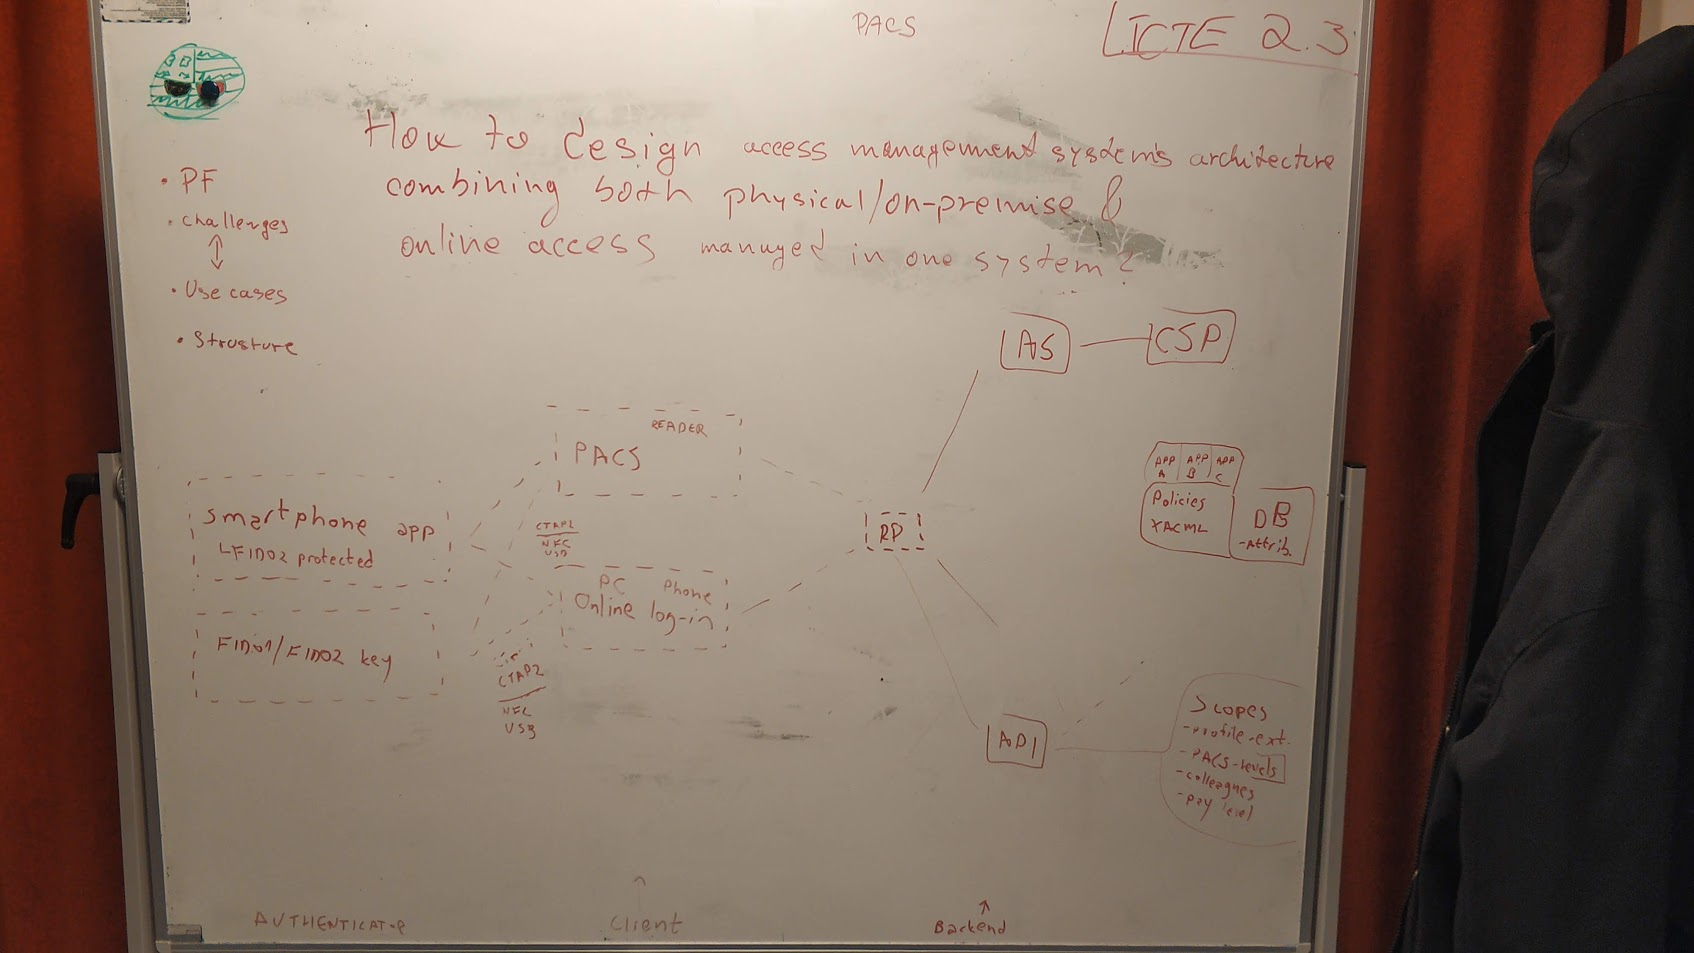
\includegraphics[width=.95\textwidth]{00images/IntroArchitecture}
    \caption{Explanation! + new diagram}
    \label{fig:IntroArchitecture}
\end{figure}

\subsection{Challenges} \label{challenges}
A number of challenges exist that will be faced in the project. The most fundamental challenge is to understand how \acrshort{ams} works, to identify its main components and to learn about the current systems. Once the knowledge is acquired, the selection of right technologies is an important aspect, as there exist many technologies and standards which can be implemented in the proposed system and therefore, finding the most suitable one is of a big importance. This goes hand in hand with designing a system’s architecture from the scratch and figuring out how the chosen components and technologies can be interconnected to perform desired tasks, while keeping in mind the security and easiness of use.

After successfully creating an architecture and choosing the right technologies, the biggest challenges starts, the implementation. In order to develop a minimum viable product/prototype XYZ, the most important components of the system have to be implemented, which requires a very good knowledge of every technology. Subsequently, a documentation of this implementation needs to be provided and decisions made during the process explained.

\subsection{Report Structure}
